\documentclass[14.5pt]{article}
\usepackage{fancyhdr}
\usepackage{listings}
\usepackage{amsmath}
\usepackage{graphicx}
\graphicspath{ {./images/} }
\pagestyle{fancy}

\lhead{Samuel Petit 17333946 petits@tcd.ie}
\rhead{Statistical Methods Final Exam}
\renewcommand{\headrulewidth}{0.4pt}
\renewcommand{\footrulewidth}{0.4pt}

\begin{document}

\section*{Question 1}
\subsection*{Part a}

We have a total of 10 topics and need to pick 3, thus the amount of possible combinations
is $\begin{pmatrix} 10 \\ 3 \end{pmatrix} = 120$.

\subsection*{Part b}

To find an expression for the probability that none of the n topics studied come up,
I first find an expression for the opposite. That is at least 1 of the topics studied
come up in the exam.
To find that expression, I use the amount of combinations possible for 3 topics drawn out
of 10. I then need to find the amount of combinations such that one or more questions out
of n studied come up. This comes down to: $\begin{pmatrix} n \\ 3 \end{pmatrix}$.
Thus, the probability that one or more questions studied come up in the exam is:
\begin{equation}
    \frac{\begin{pmatrix} n \\ 3 \end{pmatrix}}{\begin{pmatrix} 10 \\ 3 \end{pmatrix}}
\end{equation}
We are looking for the opposite thus the probability that none of the n studied topics come up is:
\begin{equation}
    1 - \frac{\begin{pmatrix} n \\ 3 \end{pmatrix}}{\begin{pmatrix} 10 \\ 3 \end{pmatrix}}
\end{equation}

\subsection*{Part c}

Knowing that the above expression gives us the probability such that no topic out of the n studied
will be in the exam, we can derive it to include two scenarios.
The first one being that all of the topics on the exam were studied. To do this we take
the number of possible combinations of topics out of the ones studied, this is
$\begin{pmatrix} n \\ 3 \end{pmatrix}$. Please not that in the case that n is less than 3,
then $\begin{pmatrix} n \\ 3 \end{pmatrix} = 0$.
To obtain the probability of this scenario happening, we divide it by the number of combinations
of exam topics that we calculated in part a: $\begin{pmatrix} 10 \\ 3 \end{pmatrix}$.

The second scenario to consider is when exactly 2 topics on the exam were studied for, to compute
this we take the number of combinations of n choose 2. And to get the number of permutations with
the 3rd non studied topic, we multiply it by $ 10 - n $

Thus this gives us the following expression for the probability of failing an exam given that n
topics were studied:
\begin{equation}
    1 - [ \frac{(10 - n) * \begin{pmatrix} n \\ 2 \end{pmatrix} + \begin{pmatrix} n \\ 3 \end{pmatrix}}{\begin{pmatrix} 10 \\ 3 \end{pmatrix}} ]
\end{equation}

We then obtain the following graph using code from appendix a.
\begin{center}
    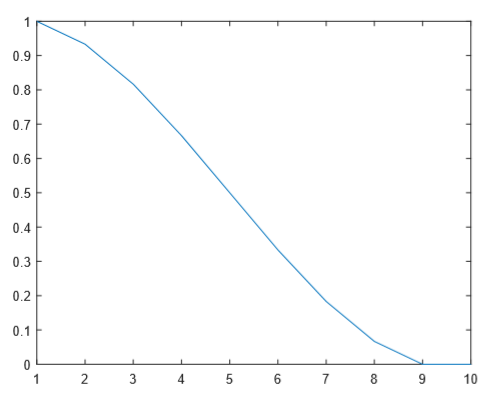
\includegraphics[scale=0.5]{p1}
\end{center}

\subsection*{Part d}
\subsection*{Part e}
\subsection*{Part f}
\subsection*{Part g}

\section*{Appendix}
\subsection*{Section a - Question 1c}
\begin{lstlisting}
%Q1 c 
y1 = zeros([1 10]);
x1 = 1:10;
% Compute the probability for all values of n
for n = x1
    y1(n) = 1 - 
        (((10-n)*
        (customNChooseK(n,2))/customNChooseK(10,3)) +
        (customNChooseK(n,3)/customNChooseK(10,3)));
end
plot(x1, y1);
\end{lstlisting}

\subsection*{Section b - Question 1d}
\begin{lstlisting}
y1 = zeros([1 10]);
x1 = 1:10;
% Compute the probability for all values of n
for n = x1
    y1(n) = 1 - (((10-n)*
    (customNChooseK(n,3))/customNChooseK(10,4))+
    (customNChooseK(n,4)/customNChooseK(10,4)) + 
    (customNChooseK(10-n,2)*(customNChooseK(n,2)/
    customNChooseK(10,4))));
end
%plot(x1, y1);

     
\end{lstlisting}

\end{document}